\begin{figure}[htbp]
    \centering
    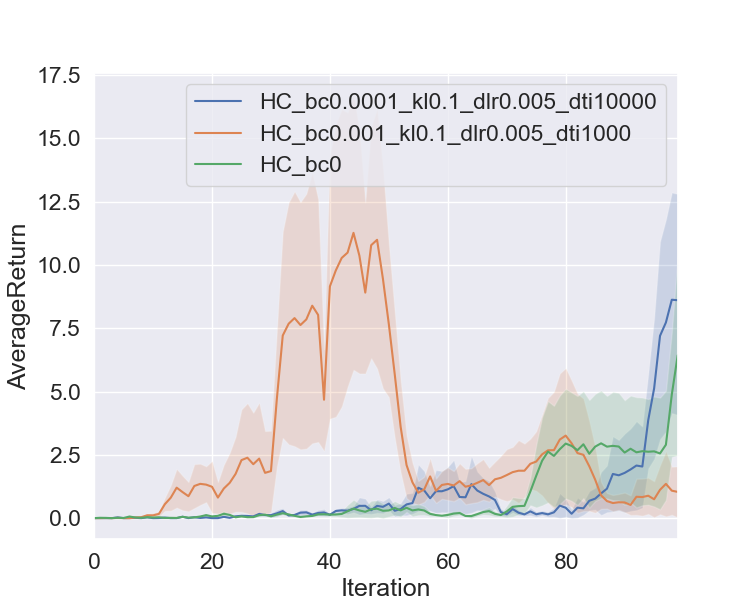
\includegraphics[width=0.5\linewidth]{figures/p4.png}
    \caption{Problem 4}
    \label{fig:p4}
\end{figure}

Please see Figure~\ref{fig:p4}. I guess with larger bonus weight the agent quickly find the best trajectory, but since it will keep visiting the optimal state, the modified reward for suboptimal states will be larger, and the behavior becomes suboptimal. With appropriate weight it learns slower but is more stable.